\documentclass[a4paper]{article}

\usepackage[english]{babel}
\usepackage[utf8]{inputenc}
\usepackage{amsmath}
\usepackage{graphicx}
\usepackage[colorinlistoftodos]{todonotes}
\usepackage{algorithm}
\usepackage[noend]{algpseudocode}
\usepackage{geometry}
\geometry{a4paper,scale=0.75}

\title{Numerical Methods in Steady State 1D and 2D Heat Equations}

\author{Yuege Xie (EID:yx4256)}
\date{}
\begin{document}
\maketitle
\tableofcontents

\newpage
\section{Introduction}
\label{sec:introduction}

The steady-state heat equation with a constant coefficient in two dimensions is given by:
$$-k\nabla^2u(x,y) = q(x,y)$$
where k is the thermal conductivity, u is the material temperature, and q is a heat source term. But in the code, I use f instead of q, it is just a notation.\\\\
In this Documentation, we first list some assumptions that help us to simplify and reformulate the 1D and 2D problems. Second, we derive the 2nd and 4th order finite difference expression using node-based central difference. Third, we transform the PDE into linear systems with certain matrices by flattening. Then, we can use Jacobi and Gauss-Seidel iterative methods to solve PDE numerically by solving linear systems. 

\section{Assumptions}
\begin{itemize}
    \item \textbf{Dirichlet Boundary Condition:} The solution is known on the boundary, i.e.
    $$ u(x)|_{x=a,b} = u_0(x)$$
    $$u(x,y)|_{\partial\Omega} = u_0(x,y)$$
    for 1D and 2D cases, respectively, hence the scheme is node-base.
    \item \textbf{Central Finite Difference Method:} use central finite difference for both 2nd order and 4th order approximations.
    \item \textbf{Special Points in 4th Order:} We assume that we know the boundary points in the case also for $i=1,N-1; j=1,N-1 $ as inputs.
    \item \textbf{Domain Size:} In 2D case, the domain is rectangular, i.e $\Omega = [a_1,b_1] \times [a_2,b_2]$. Moreover, if $b_1-a_1 = b_2-a_2$, it's square, we consider this case.
    \item \textbf{Mesh Size:} $\Delta x = \Delta y = h$, i.e. using square mesh.
    \item \textbf{Scheme:} The computational scheme is node-based.
    \item \textbf{Smoothness:} u is smooth enough that we can do the Taylor expansion.
\end{itemize}

\section{Steady State Heat Equation Numerical Formulation}
\subsection{Governing Equations}
\subsubsection{1D Case}
Using assumptions above, we can reformulate 1D steady-state heat equation with dirichlet boundary condition into:
\begin{equation}
    -k\nabla^2u(x) = q(x), ~~\forall x\in \Omega = [a,b]
\end{equation}

\begin{equation}
    u(a) = u_0(a), ~~u(b) = u_0(b)
\end{equation}

\subsubsection{2D Case}
Using assumptions above, we can reformulate 2D steady-state heat equation with dirichlet boundary condition into:
\begin{equation}
    -k\nabla^2u(x,y) = q(x,y), ~~(x,y)\in \Omega = [a_1,b_1] \times [a_2,b_2]
\end{equation}
\begin{equation}
    u(x,y)|_{\partial\Omega} = u_0(x,y)
\end{equation}

\subsection{Generate Grid Points}
For 1D case, assume we have $N+1$ points, and let $h=\Delta x$, then 
    $$x_i = a + i*h, i = 0,1,2,...,N$$
    
\begin{figure}[htbp]
\centering
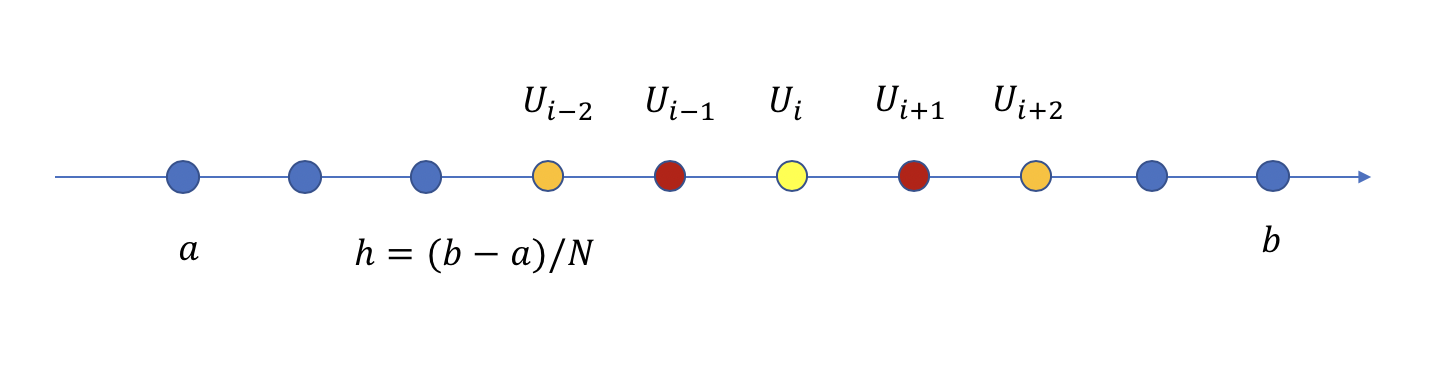
\includegraphics[width=0.8\textwidth]{1d.png}
\caption{\label{1d}Node-based 1D discretized mesh}
\end{figure}

Let $\Delta x = \Delta y = h = \frac{b_i-a_i}{N_i}$ be the distance between two grid points. Indeed, for rectangular domain, we only have to choose different $N_1$ and $N_2$ to get the same $h$. Then
$$x_i = a_1 + i*h, i = 0,1,2,...,N$$
$$y_j = a_2 + j*h, i = 0,1,2,...,N$$
We want to get approximations of $U_{ij} = u(x_i,y_j)$ at grid points $(x_i, y_j)$. Since by Dirichlet Boundary Condition, the solution on boundaries are known, we only have $(N-1)\times (N-1)$ unknowns to solve.

\begin{figure}[htbp]
\centering
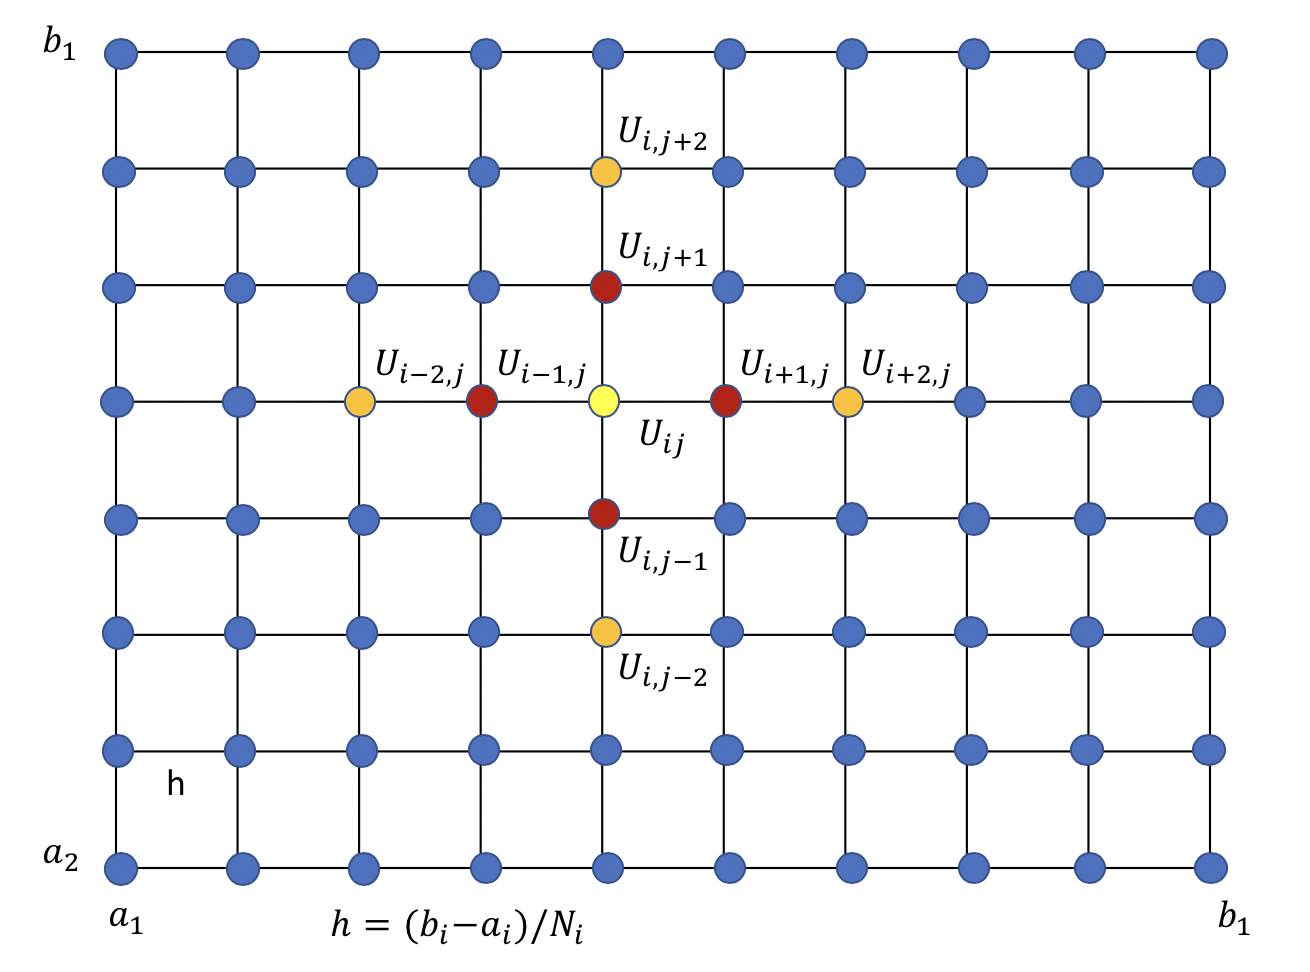
\includegraphics[width=0.8\textwidth]{2d.png}
\caption{\label{2d}Node-based 2D discretized mesh}
\end{figure}

\subsection{2nd-order Finite Difference Approximation}
\subsubsection{1D Case}
Derived from Taylor expansion of u(x,y), we have
\begin{equation}
    \begin{split}
    \nabla^2u(x_i) = & \frac{u(x_{i-1}) - 2u(x_i) + u(x_{i+1})}{h^2} -\frac{2h^2}{4!}\frac{d^4 u}{d x_i^4} + O(h^4)\\ 
    = & \frac{U_{i-1} - 2U_{i} + U_{i+1} }{h^2} + T_{i}
    \end{split}
\end{equation}

where the local truncation error $T_{i} = -\frac{2h^2}{4!}\frac{d^4 u}{d x_i^4} + O(h^4)$ and we have $\lim_{h\rightarrow 0} T_{i} = 0, \forall i,j$, we can get the following equation:

\begin{equation}
   \frac{-k}{h^2} [U_{i-1} - 2U_{i} + U_{i+1}]   = q_{i}
\end{equation}
where $q_i = q(x_i)$,  $i = 1,2,...,N-1$.

\subsubsection{2D Case}
Derived from Taylor expansion of u(x,y), we have

\begin{equation}
    \begin{split}
    \nabla^2u(x_i, y_j) = & \frac{u(x_{i-1},y_j) - 2u(x_i,y_j) + u(x_{i+1},y_j)}{h^2} + \frac{u(x_i,y_{j-1}) - 2u(x_i,y_j) + u(x_i,y_{j+1})}{h^2} \\
    & -\frac{2h^2}{4!}(\frac{\partial^4 u}{\partial x_i^4} + \frac{\partial^4 u}{\partial y_j^4}) + O(h^4)\\ 
    = & \frac{U_{i-1,j} + U_{i+1,j} + U_{i,j-1} + U_{i,j+1} - 4U_{ij} }{h^2} + T_{ij}
    \end{split}
\end{equation}

where the local truncation error $T_{ij} = -\frac{2h^2}{4!}(\frac{\partial^4 u}{\partial x_i^4} + \frac{\partial^4 u}{\partial y_j^4}) + O(h^4)$ and we have $\lim_{h\rightarrow 0} T_{ij} = 0, \forall i,j$, we can get the following equation:

\begin{equation}
   \frac{-k}{h^2} [U_{i,j-1} + U_{i-1,j} - 4U_{ij} + U_{i+1,j} + U_{i,j+1}]   = q_{ij}
\end{equation}

where $ i = 1,2,...,N-1, j = 1,2,...,N-1$ and $q_{ij} = q(x_i,y_j)$

\subsection{4th-order Finite Difference Approximation}

\subsubsection{1D Case}
\begin{equation}
    \nabla^2 u(x_i) = \frac{-U_{i-2,j} + 16U_{i-1,j} - 30U_{ij} + 16 U_{i+1,j} - U_{i+2,j}}{12h^2} -\frac{8h^4}{6!}\frac{d^6 u}{d x_i^6}  + O(h^6)
\end{equation}

where $\lim_{h\rightarrow 0} -\frac{8h^4}{6!}\frac{d^6 u}{d x_i^6}  + O(h^6) = 0, \forall i$. Then we get:
\begin{equation}
    \frac{-k}{h^2}[ -\frac{1}{12}U_{i-2} + \frac{4}{3}U_{i-1} - \frac{5}{2}U_{i} + \frac{4}{3}U_{i+1} - \frac{1}{12}U_{i+2}] = q_{i}
\end{equation}

where $ i = 2,...,N-2$ and $q_{i} = q(x_i)$. 

\subsubsection{2D Case}
Similar as above, ignore the high order term of $h$, we have 
\begin{equation}
    \begin{split}
    \nabla^2 u(x_i, y_j) =  & \frac{-U_{i-2,j} + 16U_{i-1,j} - 30U_{ij} + 16 U_{i+1,j} - U_{i+2,j}}{12(\Delta x)^2}\\
    & + \frac{-U_{i,j-2} + 16 U_{i,j-1} - 30 U_{i,j} + 16U_{i,j+1} -U_{i, j+2} }{12(\Delta y)^2}  + T_{ij}
    \end{split}
\end{equation}

where the local truncation error $T_{ij} = -\frac{8h^4}{6!}(\frac{\partial^6 u}{\partial x^6} + \frac{\partial^6 u}{\partial y^6}) + O(h^6) $ $\lim_{h\rightarrow 0} T_{ij} = 0, \forall i,j$ as well, we can get the equations:
\begin{equation}
    \frac{-k}{h^2}[ -\frac{1}{12}U_{i-2,j} + \frac{4}{3}U_{i-1,j} - 5U_{ij} + \frac{4}{3} U_{i+1,j} - \frac{1}{12}U_{i+2,j} -\frac{1}{12}U_{i,j-2} + \frac{4}{3} U_{i,j-1} + \frac{4}{3}U_{i,j+1} -\frac{1}{12}U_{i, j+2}] = q_{ij}
\end{equation}

where $ i = 2,...,N-2, j = 2,...,N-2$ and $q_{ij} = q(x_i,y_j)$.

\subsection{Linear System of Heat Equation and Matrix Form}
\subsubsection{1D Case}
For 1D case, just let $z=[U_0, U_1,...,U_{N-1},U_N]^T$, where $U_0=u_0(a), U_N=u_0(b)$, then we can get the $Az = b$ form, which can be solved by iterative methods. For 2nd order approximation, with Dirichlet boundary conditions known, we have the following form:
$$b_{2nd}^{1D} = [ U_0, q_1,...,q_{N-1}, U_N ]^T$$

\[
A_{2nd}^{1D}
= \frac{-k}{h^2}
\begin{bmatrix}
    
    \frac{-h^2}{k}  &  &   & & & \\
    1  & -2 & 1  &   &  &\\
       & 1  & -2 & 1  &  & \\
     & & \ddots & \ddots & \ddots & & \\
     & & & 1 & -2  & 1&\\
     & & &  &  & \frac{-h^2}{k} \\
\end{bmatrix}
\]
\#nonzeros of interior: 3, except first and last is 1.  \\
\textbf{Note:} Since for boundary points, we only need 1 for it, to make the matrix simple, I add $\frac{-h^2}{k}$ to recover it to 1.

For 4th order approximation, 
$$b_{4th}^{1D} = [ U_0, U_1, q_2,...,q_{N-2}, U_N-1,U_N ]^T$$

\[
A_{4th}^{1D}
= \frac{-k}{h^2}
\begin{bmatrix}
    
    \frac{-h^2}{k}   &  &   & & & &\\
       & \frac{-h^2}{k} &   &   &  & &\\\\
     -\frac{1}{12}  & \frac{4}{3}  & -\frac{5}{2} & \frac{4}{3}  & - \frac{1}{12} & &&\\
     & \ddots& \ddots & \ddots & \ddots & \ddots & \\
    && -\frac{1}{12}  & \frac{4}{3}  & -\frac{5}{2} & \frac{4}{3}  & - \frac{1}{12} \\\\
     & & & &  &  \frac{-h^2}{k}  & \\
     & & & &  & &\frac{-h^2}{k}  \\
\end{bmatrix}
\]
\#nonzeros of interior row: 5, except first, second, first last and second last is 1.

\subsubsection{2D Case}
We want to transform the 2D problem into a linear system $Az=b$ as well and use iterative methods like Jacobi and Gauss-Seidel to solve it.
First, assume $N_1=N_2=N$, flatten $U_{ij}$ into a vector $z$ using rule: 
$$z_{i(N+1)+j} = U_{i,j}, \forall i = 0,1,2,...N, j = 0,1,2,...,N$$
Then we have $z = [U_{00}, U_{01},...,U_{0N},U_{10},...,U_{NN}]^T$.  \\
Second, we use the same rule of adding boundary variables as 1D case to flatten $f$ into $b$:
$$b_{2nd}^{2D} = [U_{00}, U_{01},..., U_{0,N}, U_{10}, q_{11},...,q_{1,N-1},...,q_{N-1,N-1},U_{N-1,N},...,U_{N,N} ]^T $$
Third, we can get the form of corresponding A:
\[
A_{2nd}^{2D}
= 
\begin{bmatrix}
     I &  &   &   &  &\\
    I_{2nd} & B_{2nd} & I_{2nd}  &   &  &\\
     & & \ddots & \ddots & \ddots & & \\
     & & & I_{2nd}& B_{2nd}  & I_{2nd}& \\
     & & &  &  &  I  \\
\end{bmatrix}
\]
where $I_{2nd}$ and $B_{2nd}$ are $N+1 \times N+1$ matrix.\\
\#nonzeros of interior row: 5, except special cases with 1. 
\[
B_{2nd} = \frac{-k}{h^2}
\begin{bmatrix}
    \frac{-h^2}{k}\\
    1 & -4 & 1  &     \\
    
     & \ddots & \ddots & \ddots  \\
     &  & 1 & -4  &1 \\
     &  &   & & \frac{-h^2}{k}\\
\end{bmatrix}
\]

\[
I_{2nd} = \frac{-k}{h^2}
\begin{bmatrix}
    0\\
      &1&  &   &     \\
    
     & & \ddots  \\
     &  &  &1 \\
     &  &   & & 0\\
\end{bmatrix}
\]

\begin{figure}[htbp]
\centering
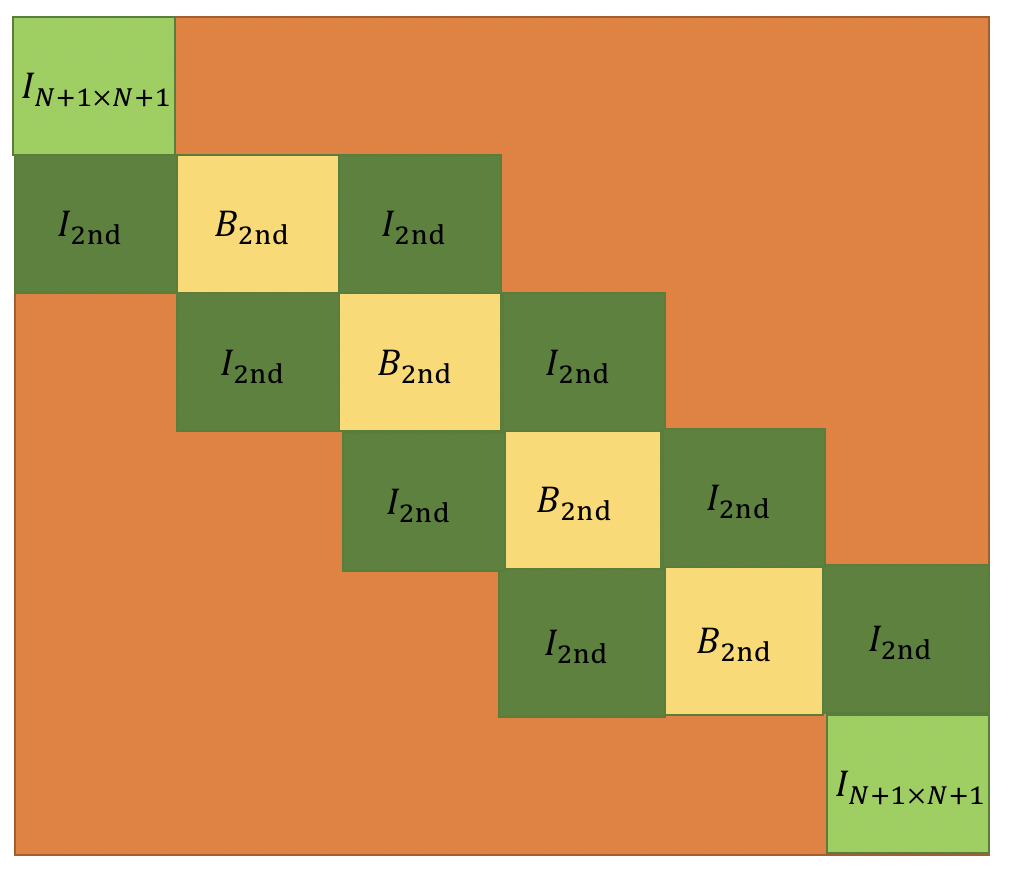
\includegraphics[width=0.7\textwidth]{2nd.png}
\caption{\label{2nd}Structure of 2nd order difference matrix}
\end{figure}

For 4th order approximation, we know more boundary conditions including $i=0,1,N-1,N;j=0,1,N-1,N$, we have:
$$b_{4th}^{2D} = [U_{00}, U_{01},..., U_{0N}, U_{10}, U_{11},...,U_{1N},U_{20},q_{21},...,q_{N-2,N-2},U_{N-1,N},...,U_{N,N} ]^T $$

\[
A_{4th}^{2D}
= 
\begin{bmatrix}
     I &  &   &   &  &\\
      &I &   &   &  &\\
    -\frac{1}{12}I_{4th}& \frac{4}{3}I_{4th} & B_{4th} & \frac{4}{3}I_{4th} & -\frac{1}{12}I_{4th} \\
      &\ddots& \ddots & \ddots & \ddots & \ddots& \\
     &&-\frac{1}{12}I_{4th}& \frac{4}{3}I_{4th} & B_{4th} & \frac{4}{3}I_{4th} & -\frac{1}{12}I_{4th} \\
     & & & & &    I \\
     & & &  & &  &  I  \\
\end{bmatrix}
\]
where $I=I_{N+1\times N+1}$ and $B$ is also $N+1 \times N+1$ matrix.\\
\#nonzeros of interior row: 9, except boundary cases are 1.

\[
B_{4th}
= \frac{-k}{h^2}
\begin{bmatrix}
     \frac{-h^2}{k} \\
    & \frac{-h^2}{k}\\\\
    -\frac{1}{12}  & \frac{4}{3}  & -5 & \frac{4}{3}  & - \frac{1}{12} & &&\\
    
     & \ddots& \ddots & \ddots & \ddots & \ddots & \\
    
    && -\frac{1}{12}  & \frac{4}{3}  & -5 & \frac{4}{3}  & - \frac{1}{12} \\\\
    &&&&& \frac{-h^2}{k} \\
    &&&&&& \frac{-h^2}{k} \\
\end{bmatrix}
\]

\[
I_{4th}
=  \frac{-k}{h^2}
\begin{bmatrix}
    0\\
    & 0\\
    &&1\\
    &&&\ddots \\
    &&&&1\\
    &&&&&0\\
    &&&&&&0\\
\end{bmatrix}
\]


\begin{figure}[htbp]
\centering
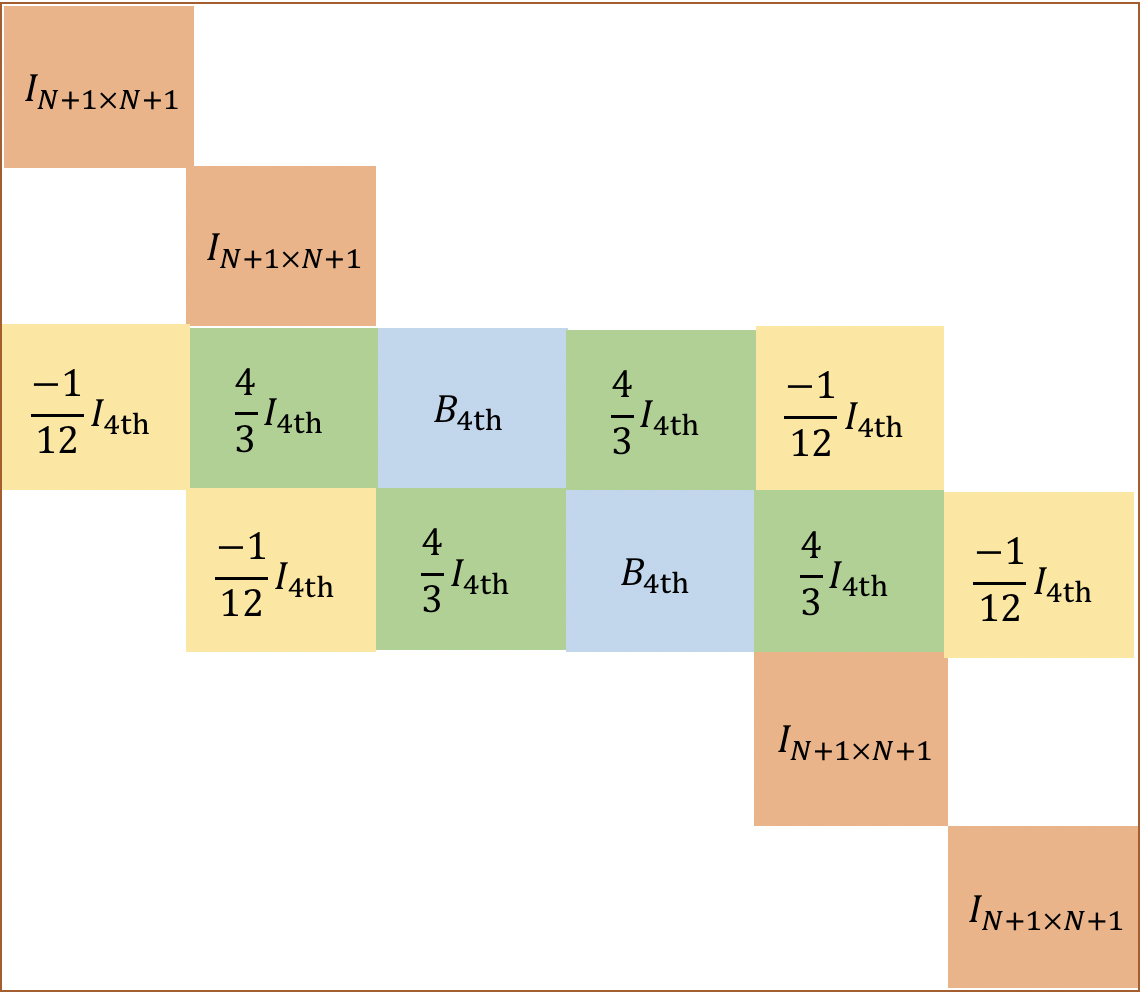
\includegraphics[width=0.7\textwidth]{4th.png}
\caption{\label{4th}Structure of 4th order difference matrix}
\end{figure}

\subsection{Iterative Methods to Solve Linear Systems}
\subsubsection{Jacobi Iterative Method}
Given an initial guess $\mathbf{z}^0 $, here we use $0$ for initialization, then the rule of Jacobi iterative method is 
\begin{equation}
    z_i^{k+1} = \frac{1}{a_{ii}}(b_i-\sum_{j=1,j\neq i}^n a_{ij}z_j^k)
\end{equation}

\subsubsection{Gauss-Seidel Iterative Method}
Given an initial guess $\mathbf{z}^0$, here we use $0$ for initialization,then the rule of Gauss-Seidel iterative method is 
\begin{equation}
    z_i^{k+1} = \frac{1}{a_{ii}}(b_i-\sum_{j=1}^{i-1} a_{ij}z_j^{k+1}-\sum_{j=i+1}^{n} a_{ij}z_j^{k})
\end{equation}

Gauss-Seidel method use the newest to solve linear system, while Jacobi use the old one. For performance, Gauss-Seidel usually converges and use less memory, but not for Jacobi. In practice, we can see from the results, Jacobi does not converge for 4th order finite difference.\\

\section{Algorithm}
\begin{algorithm}
\caption{Numerical Methods to Solve Steady State Heat Equations}
    \begin{algorithmic}
    \State \textbf{Input:} tolerance $\epsilon >0$, max\_iter, iter\_method, dim, fd\_method, domain, $N$, dim, output\_mode, verification\_mode, output\_file
    \State \textbf{Output:} $u(x_i,y_j), i = 1,2,...,N-1, j = 1,2,...,N-1$ 
    \State \textbf{Initialize:} k = 0, error = 1000, $f(x_i,y_j)$
        \If{dim == 1}
            $$z=[U_0, U_1,...,U_{N-1},U_N]^T$$
            
            \If{fd\_method == 2nd}
            $$b = b_{2nd}^{1D}$$
            $$A = A_{2nd}^{1D}$$
            \Else
            $$b = b_{4th}^{1D}$$
            $$A = A_{4th}^{1D}$$
            \EndIf
        \EndIf
        
        \If{dim == 2} 
             $$z = [U_{00}, U_{01},...,U_{0N},U_{10},...,U_{NN}]^T$$
            \If{fd\_method == 2nd}
            $$b = b_{2nd}^{2D}$$
            $$A = A_{2nd}^{2D}$$
            \Else
            $$b = b_{2nd}^{2D}$$
            $$A = A_{4th}^{2D}$$
            \EndIf
        \EndIf
    
        \While { error $> \epsilon$ and k $<=$ max\_iter }
        
        
        \If {iter\_method == Jacobi}
        \For {$i=0,1,2,..,N$}
        sum = 0
        \For {$j=0,1,2,...,N$}
        \If{$j\neq i$}
        $sum = sum+a_{ij}z_j^k$
        \EndIf
        \EndFor
        $z_i^{k+1} = \frac{1}{a_{ii}}(b_i-sum)$
        \EndFor
        \EndIf
        
        
        \If {iter\_method == Gauss\_Seidel}
        \For {$i=0,1,2,..,N$}
        sum = 0
        \For {$j=0,1,2,...,i-1$}
        $sum = sum+a_{ij}z_j^{k+1}$
        \EndFor
        \For {$j=i+1,i+2,...,N$}
        $sum = sum+a_{ij}z_j^k$
        \EndFor
        $z_i^{k+1} = \frac{1}{a_{ii}}(b_i-sum)$
        \EndFor
        \EndIf
         
        \If {iter\_method == GMRES}
            use PETSC to get solution
        \EndIf
        \State error = $\|z^{k+1}-z^k\|_2$
        \State $k \leftarrow k+1$
        \EndWhile
    \Return $z^k$
    \end{algorithmic}
\end{algorithm}

\section{Memory Estimate}
Memory that we need includes the following things:
\begin{itemize}
    \item \textbf{Iteration Variables:} matrix A, vector b, vector z, $k$, error
    \item \textbf{Inputs:} tolerance $\epsilon$, max\_iter, iter\_method, dim, fd\_method, domain, $N$, output\_mode, verification\_mode, output\_file
\end{itemize}

\begin{enumerate}
    \item For matrix A, because it has special diagonal structures, we can use sparse structure to store it. Use 1D array to save number of non-zeros in each row, let $n = N+1$ for 1D case and $n = (N+1)*(N+1)$ for 2D case. Then we need $n$ for non-zeros. Use 2D array to save non-zero column index and values, we need $3n$ for 1D 2nd, $5n$ for 1D 4th and 2D 2nd, $9n$ for 2D 4th.
    \item For inputs and iteration variables $k$, error, we only need 1 double to store them, we can estimate 20 doubles for them.
    \item For z and b, we need $N+1$ for 1D case and $(N+1)^2$ for 2D case, respectively.
    \item For verification mode, we need $n$ for exact value.

\end{enumerate}

The difference between Jacobi and Gauss-Seidel iterations is that we update the variable in Gauss-Seidel iteration in the loop, so we only need one z to store it. But for Jacobi, we update them until we get all the new values for a new iteration, so we need at least two z to store them. But we need to compare the $l2$ norm for current and previous solution, so here we need one more $n$ doubles for "old\_z".

And we need 8B to store a double, then the total memory we need is as follows in Table \ref{table}. And we allocate dynamic memory to these variables.

\begin{table}[htbp]
\centering
\begin{tabular}{l|l|lll}
\hline
iter\_method/dim & 1D & 2D \\
\hline
2nd order & $(11\times (N+1)+ 20)\times 8B$ & $(15\times (N+1)^2+ 20)\times 8B$   \\
4th order & $(15\times (N+1)+ 20)\times 8B$ & $(23\times (N+1)^2+ 20)\times 8B$  \\
\hline
\end{tabular}
\caption{\label{table}Memory Estimate Summary}
\end{table}

\newpage
\section{User Instructions}
\subsection{Build Procedures}
Please follow the procedures to build heat equation solving systems on Stampede2,and the commands are also include in \textbf{"build\_coverage.sh"} and \textbf{"build\_petsc.sh"}, you can use "cat build\_coverage.sh" and copy the commands for convenience.\\
Since the two can not be build at the same time, I strongly recommend you to build coverage at first, and use "make coverage" to get the coverage results, then build with PETSC to see other related results.\\\\
\textbf{To enable coverage option, you can build as follows:}
\begin{enumerate}
    \item Download the tar of codes, "proj02" from Github, untar the files;
    \item Use "autoreconf -f -i" to do the bootstrap;
    \item Export PATHs;
    \begin{verbatim}
    export PKGPATH=/work/00161/karl/stampede2/public
    export CLASSPATH=/work/00161/karl/stampede2/public
    export MODULEPATH=$CLASSPATH/ohpc/pub/modulefiles/:$MODULEPATH
    \end{verbatim}
    \item Load fixed toolchain, and use "which gcc" to check if the version is "/work/00161/karl/stampede2/public/ohpc/pub/compiler/gcc/7.1.0/bin/gcc"
    \begin{verbatim}
    module swap intel gnu7
    \end{verbatim}
    \item Load hdf5 module;
    \begin{verbatim}
    module load hdf5
    \end{verbatim}
    \item Use the following command to do the configuration;
    \begin{verbatim}
    ./configure CC=gcc --with-masa=$PKGPATH/masa-gnu7-0.50 \
    --with-grvy=$PKGPATH/grvy-gnu7-0.34 \
    --with-hdf5=$TACC_HDF5_DIR --enable-coverage
    \end{verbatim}
    \item Use "make" to automatically build the system and "make check" to check it runs correctly;
    \item Use "make coverage" to see the percentage of lines used in check process;
    \item Use "cd src" to enter in the src file and "./solver input.dat" to solve heat equation, where you can change input.dat following the instructions in the file, which will also be illustrated in the "Input Options".
\end{enumerate}

\textbf{To enable PETSC option, you can build as follows:}
\begin{enumerate}
    \item Follow steps 1,2,3 the same as above and if you have built as above, remember to "make clean";
    \item Load hdf5 and petsc modules;
    \begin{verbatim}
    module load hdf5
    module load petsc
    \end{verbatim}
    \item Use the following command to do the configuration;
    \begin{verbatim}
    ./configure CC=mpicc --with-masa=$PKGPATH/masa-gnu7-0.50 \
    --with-grvy=$PKGPATH/grvy-gnu7-0.34 \
    --with-hdf5=$TACC_HDF5_DIR --with-petsc=$PETSC_DIR
    \end{verbatim}
    \item Follow step 7 above to "make" and "make check";
    \item Use step 9 to run, but you should use mpirun on computational node as follows:
    \begin{verbatim}
    srun --pty -N 1 -n 48 -t 15:00 -p skx-dev /bin/bash -l
    mpirun -np 1 ./solver input.dat
    \end{verbatim}
\end{enumerate}

\subsection{Input Options}
Input options can be changed in input.dat, which shows in Figure \ref{input}.
Note that you can also change the name and the file name on the command line.

\begin{itemize}
    \item k: thermal conductivity, which will be used as parameter for MASA
    \item verify\_mode: 1 will enable verification mode with MASA and output error norm
    \item output\_ mode: 0 = silent, 1 = standard, 2 = debug
    \item output\_file: name of solution output file, for "make check", please set it as "sol.dat"
    \item dimensions: choose 1 for 1D and 2 for 2D
    \item xmin, xmax, ymin, ymax: set range of each axis
    \item N: number of intervals in one axis, points are $N+1$ for 1D, $(N+1)^2$ for 2D.
    \item fd\_method: 2 = second order, 4 = fourth order
    \item iter\_method: choose 1 for Jacobi or 2 for Gauss-Seidel or 3 for GMRES using PETSC
    \item eps: iterative solver tolerance, default is $1.0e-12$
    \item max\_iter: max solver iterations
\end{itemize}

\begin{figure}[htbp]
\centering
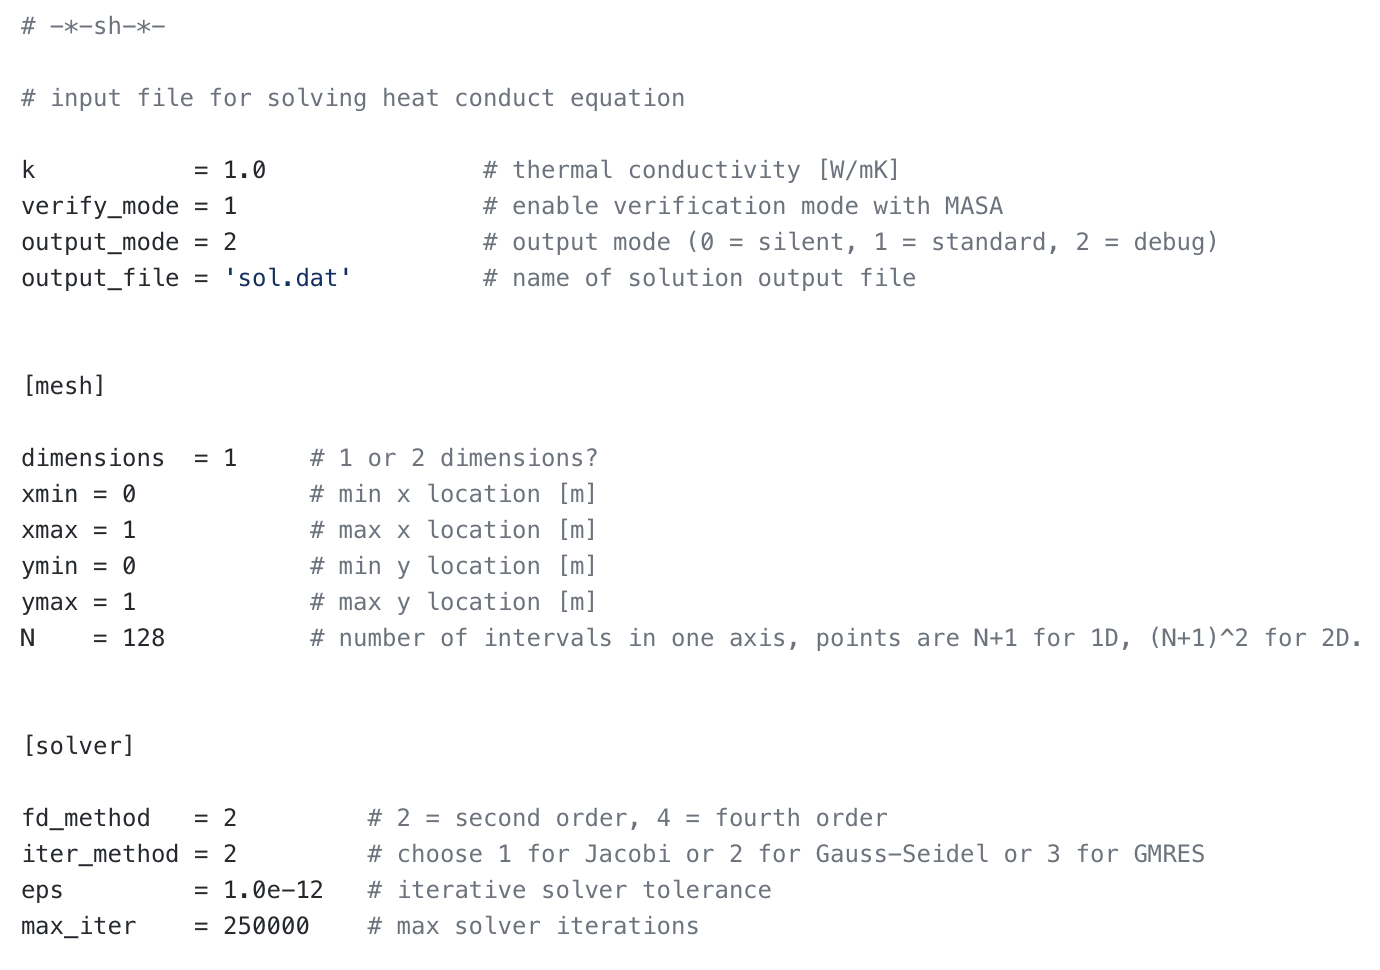
\includegraphics[width=0.8\textwidth]{input.png}
\caption{\label{input}Input options example}
\end{figure}

\newpage
\section{Code Coverage}
We can use "make coverage" without PETSC and get the coverage results in the directory \textbf{"/coverage/lcov"} and Figure \ref{coverage}. You can check the "*.html" to see overall and detailed information.
As we can see from the figure, the regression tests have $95.9\%$ code coverage, which is bigger than $75\%$.
And you can also see on the screen. \\
\begin{verbatim}
"Overall coverage rate:
  lines......: 95.9% (374 of 390 lines)
  functions..: 100.0% (7 of 7 functions)"
\end{verbatim}
\begin{figure}[htbp]
\centering
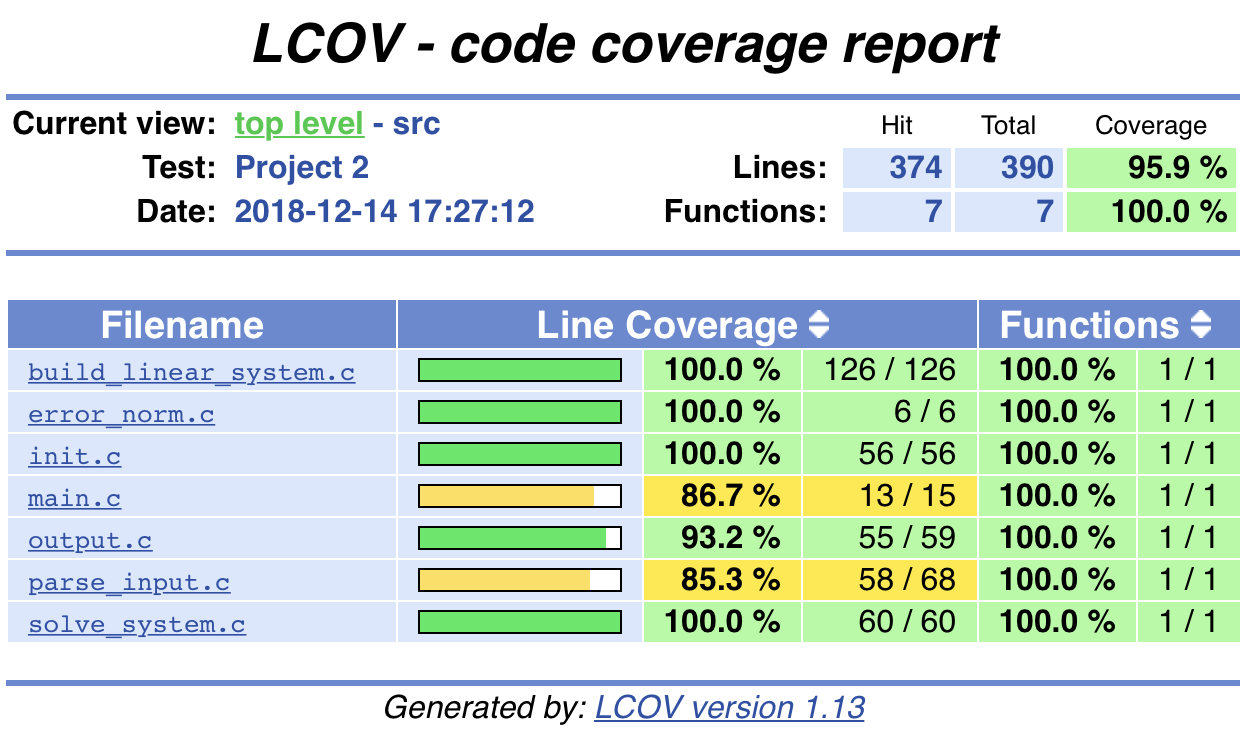
\includegraphics[width=0.9\textwidth]{coverage.png}
\caption{\label{coverage}Code Coverage Demonstration}
\end{figure}

\section{Verification Procedures and Exercise}
Just change the input.dat with verify\_mode to run in verification mode, since the silent output mode will show nothing, please change the output\_mode to 1 or 2 to see the $l_2$ norm for the difference between the solution and the reference result generated from MASA. You can find example output for standard output in Figure \ref{std_v}, for debug output in Figure \ref{debug_v}.\\\\
For verification exercise, we can run with $N= 8, 16, 32, 64, 128, 256$, and use "loglog" to plot and to illustrate the convergence rate with reference line. The expected slope for 2nd order is $-2$ and for 4th order is $-4$. We can see the result of Gauss-Seidel iterative method for 1D and 2D in Figure \ref{gauss_1d} and Figure \ref{gauss_2d}, respectively; and Jacobi iterative method for 1D and 2D with 2nd order in Figure \ref{jacobi}. They are all almost parallel to the reference line respectively.\\\\
From the results we can get slope as follows, Gauss and Jacobi are close in 2nd order.\\
\begin{itemize}
    \item 1d 2nd gauss:  -2.0238
    \item 1d 4th gauss:  -3.8642
    \item 2d 2nd gauss:  -1.9933
    \item 2d 4th gauss:  -3.8663
    \item 1d 2nd jacobi: -2.0038
    \item 2d 2nd jacobi: -1.9933
\end{itemize}

\begin{figure}[htbp]
\centering
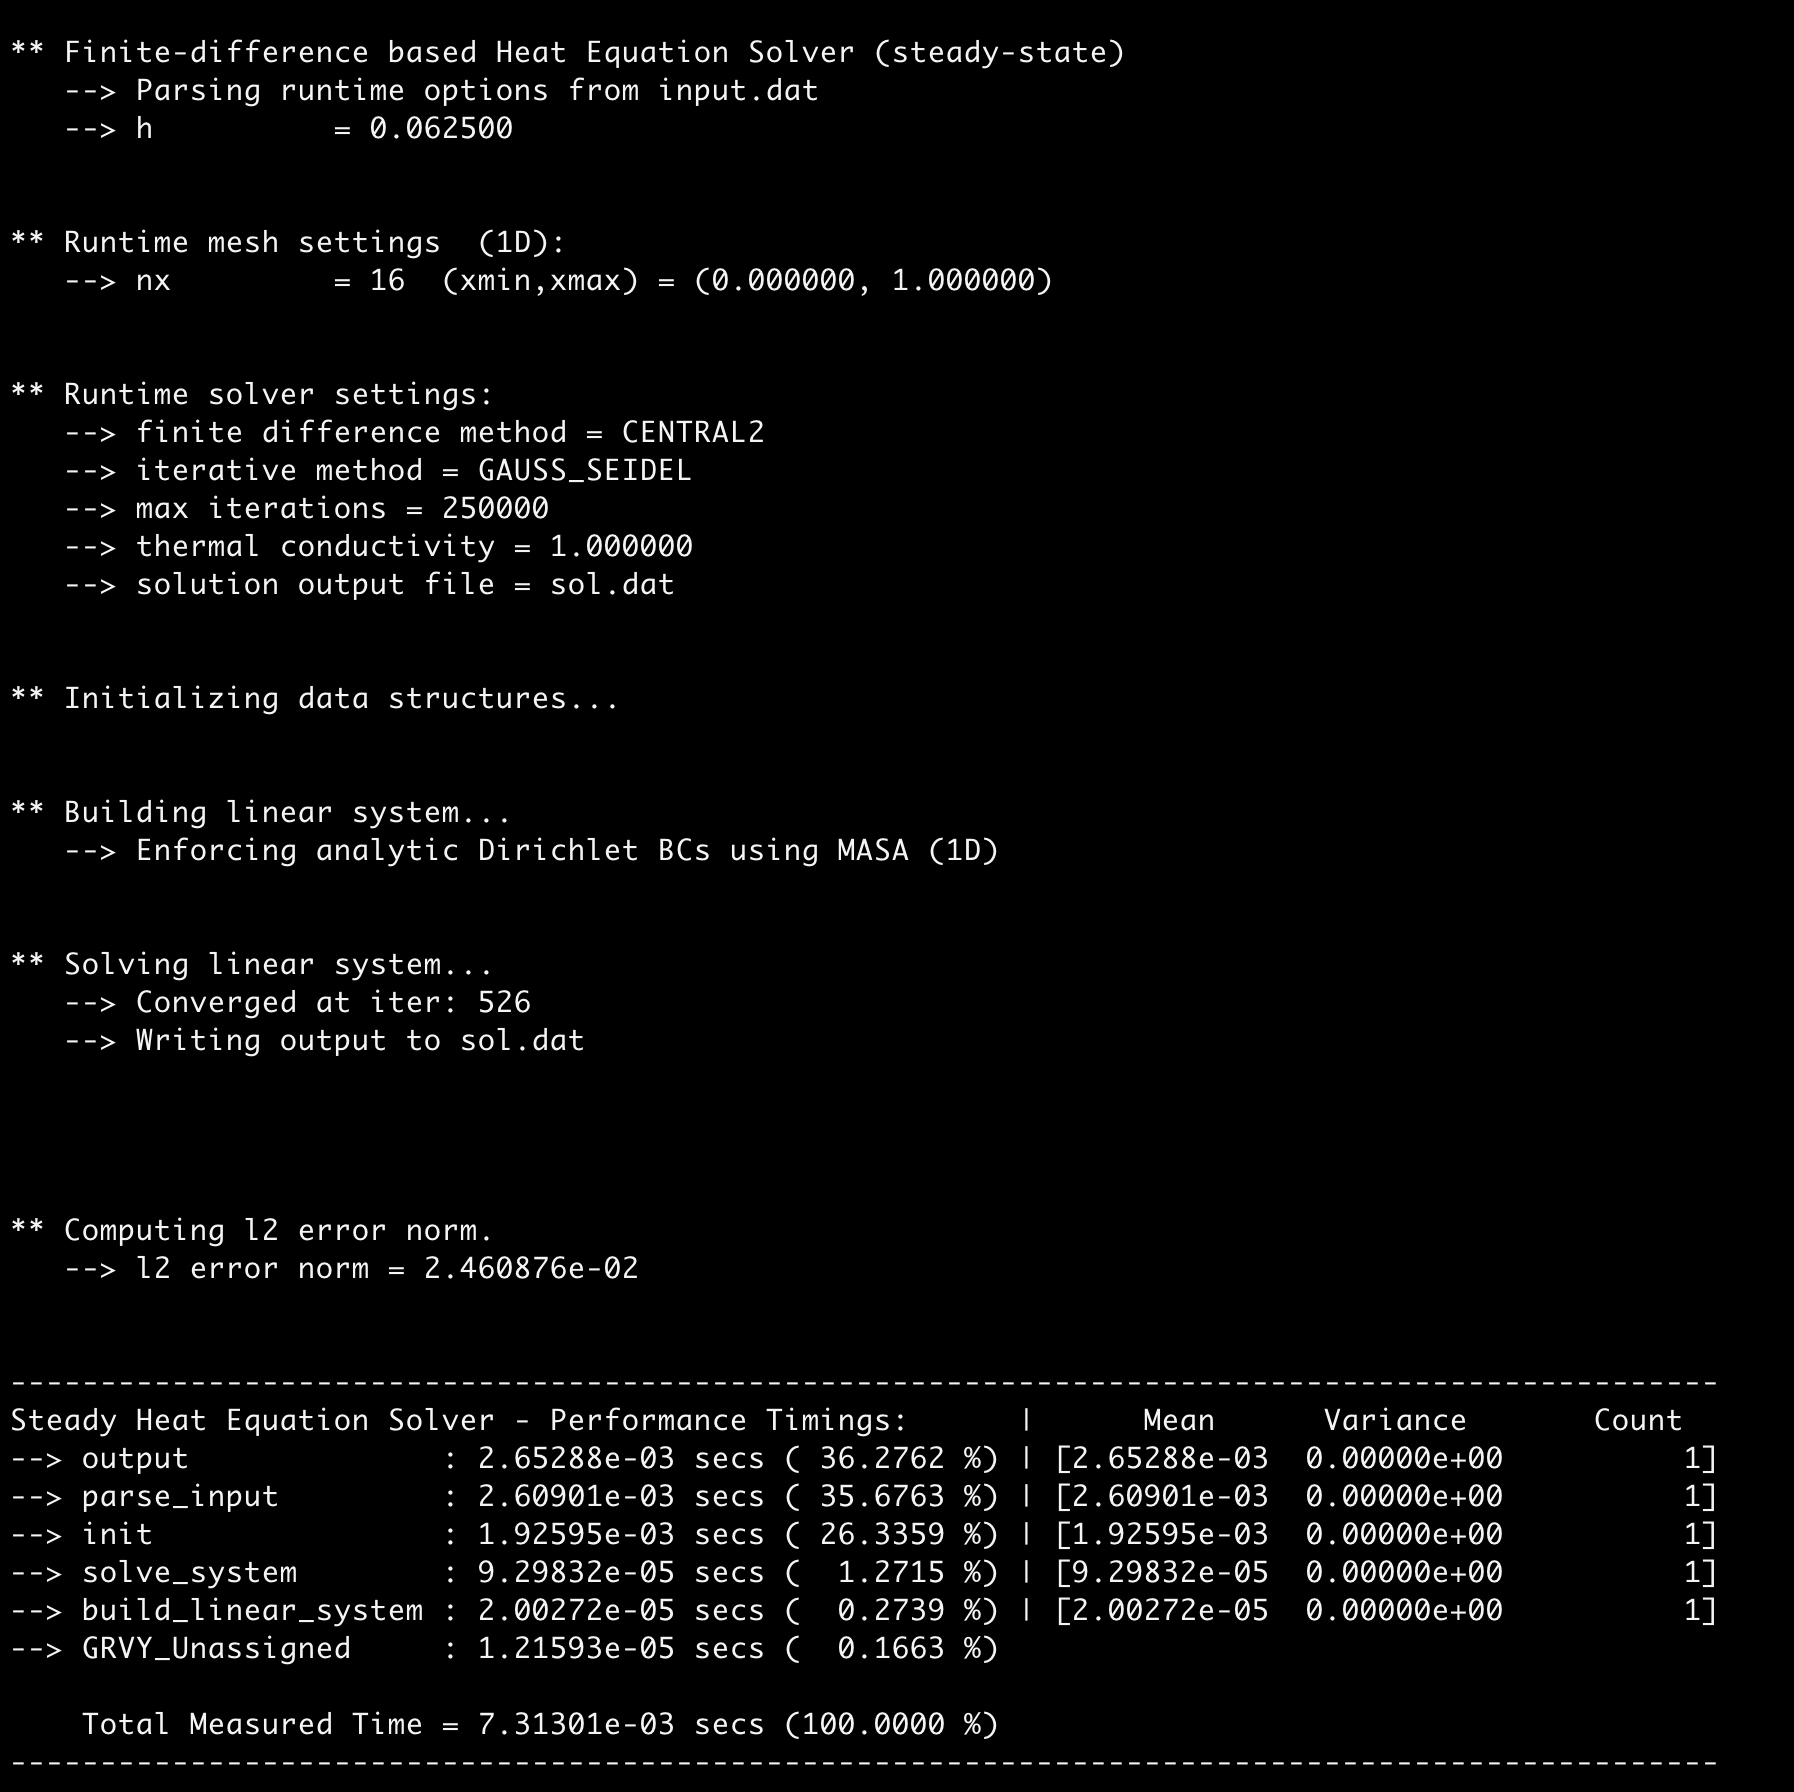
\includegraphics[width=1\textwidth]{example.png}
\caption{\label{eg}Example of standard output for verification}
\end{figure}

\begin{figure}[htbp]
\centering
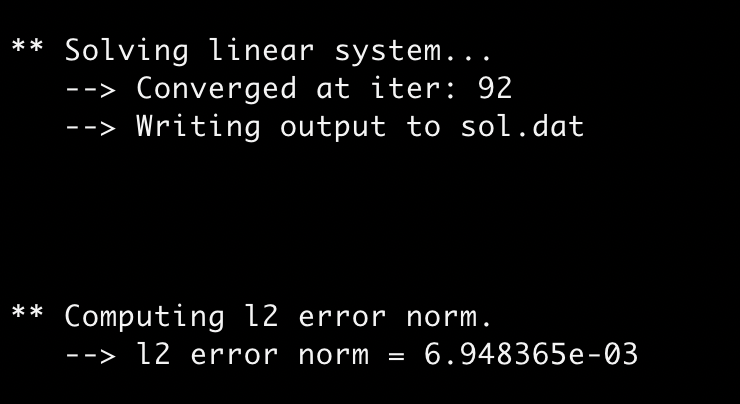
\includegraphics[width=0.4\textwidth]{std_v.png}
\caption{\label{std_v}Standard for verification}
\end{figure}

\begin{figure}[htbp]
\centering
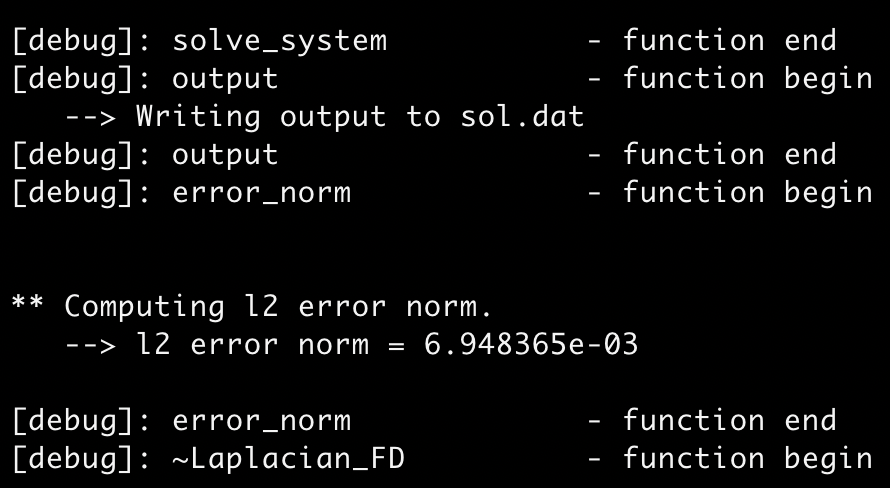
\includegraphics[width=0.4\textwidth]{debug_v.png}
\caption{\label{debug_v}Debug for verification}
\end{figure}

\begin{figure}[htbp]
\centering
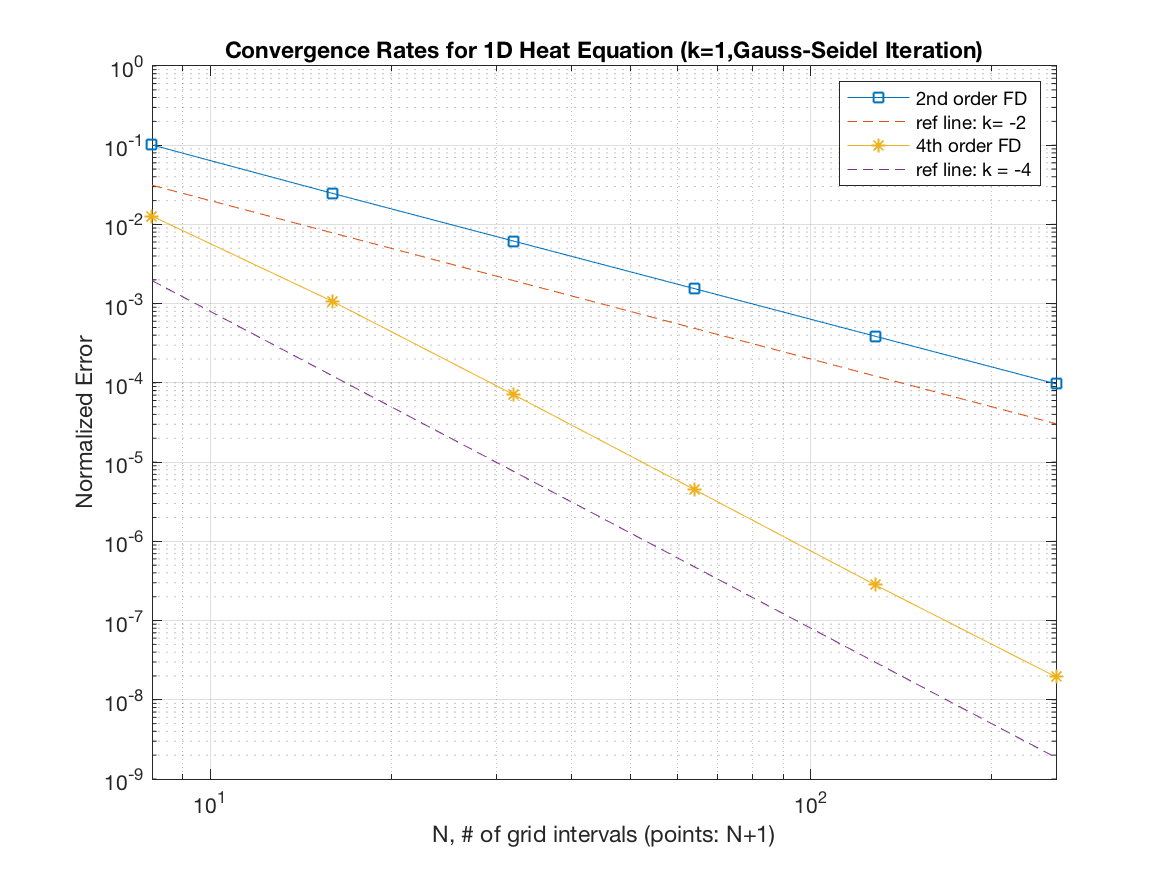
\includegraphics[width=0.8\textwidth]{gauss_1d.png}
\caption{\label{gauss_1d}Convergence Rates for 1D Heat Equation with Gauss-Seidel}
\end{figure}

\begin{figure}[htbp]
\centering
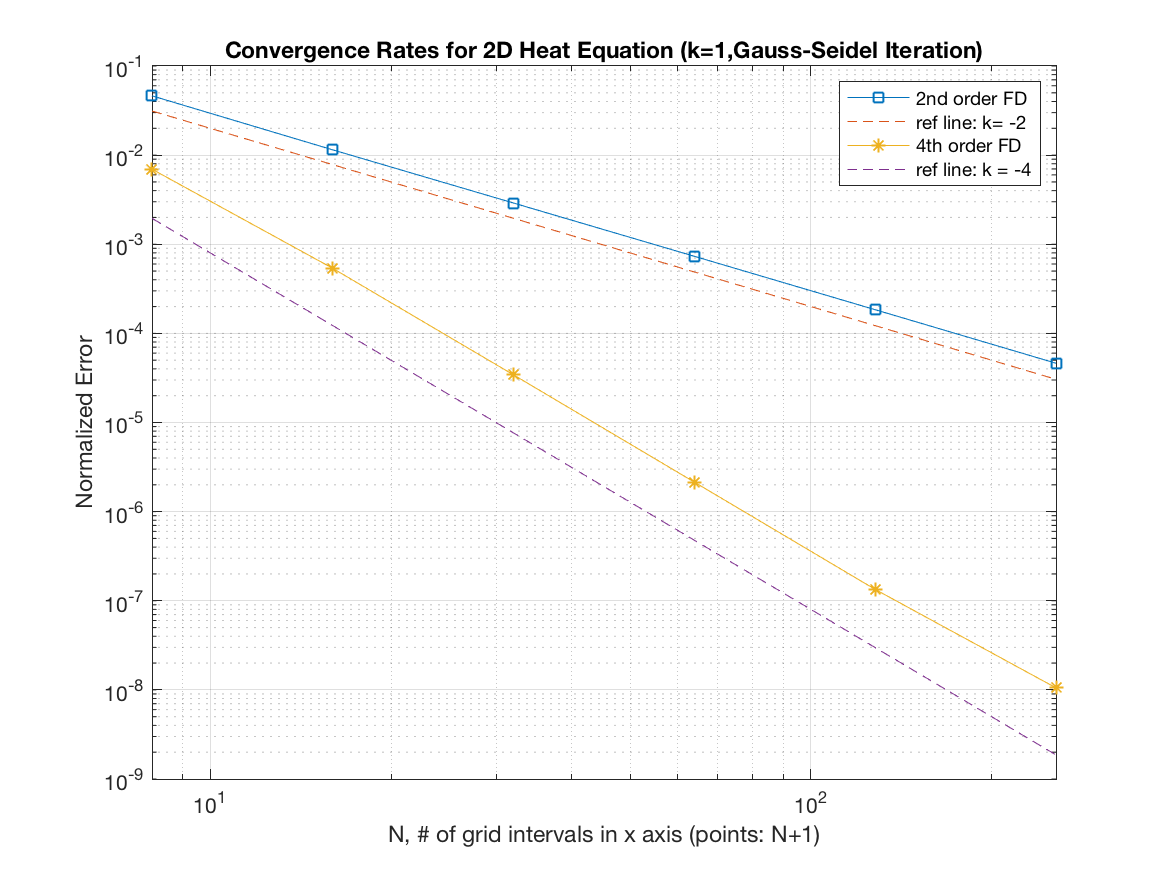
\includegraphics[width=0.8\textwidth]{gauss_2d.png}
\caption{\label{gauss_2d}Convergence Rates for 2D Heat Equation with Gauss-Seidel}
\end{figure}

\begin{figure}[htbp]
\centering
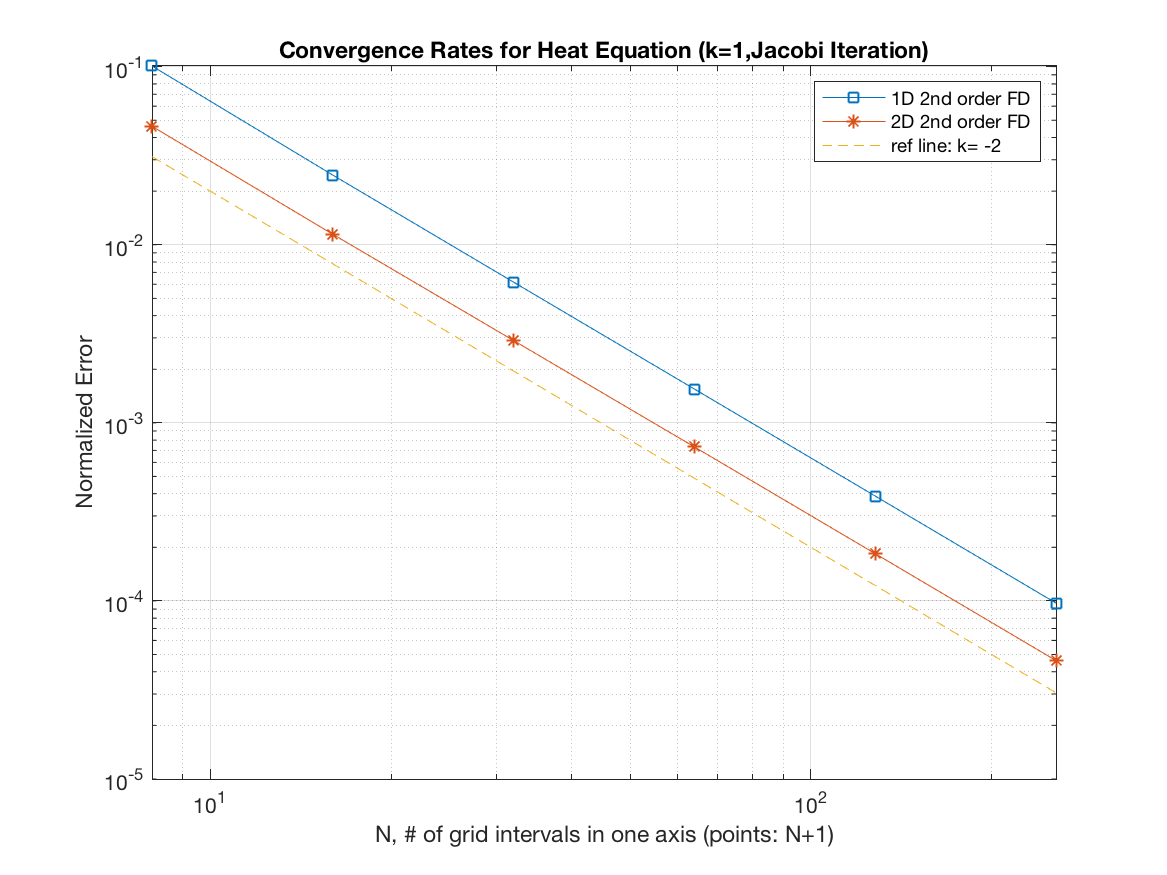
\includegraphics[width=0.8\textwidth]{jacobi.png}
\caption{\label{jacobi}Convergence Rates for Heat Equation with Jacobi}
\end{figure}

\section{Runtime Performance}
We use "GRVY" to get the summary of application time. As we can see from Figure \ref{run8}, the 3 sections accounting for at least $90\%$ are: parse\_input, init and output, since the number of points are very small and solving process is very fast, the time spends more on read and output files. From Figure \ref{run32}, the top three are solver\_system parse\_input and output, as the number of points rises, more time will spend on solver system procedure. When the number of points arrives at 256, over $99\%$ time spends on solving procedure.

\begin{figure}[htbp]
\centering
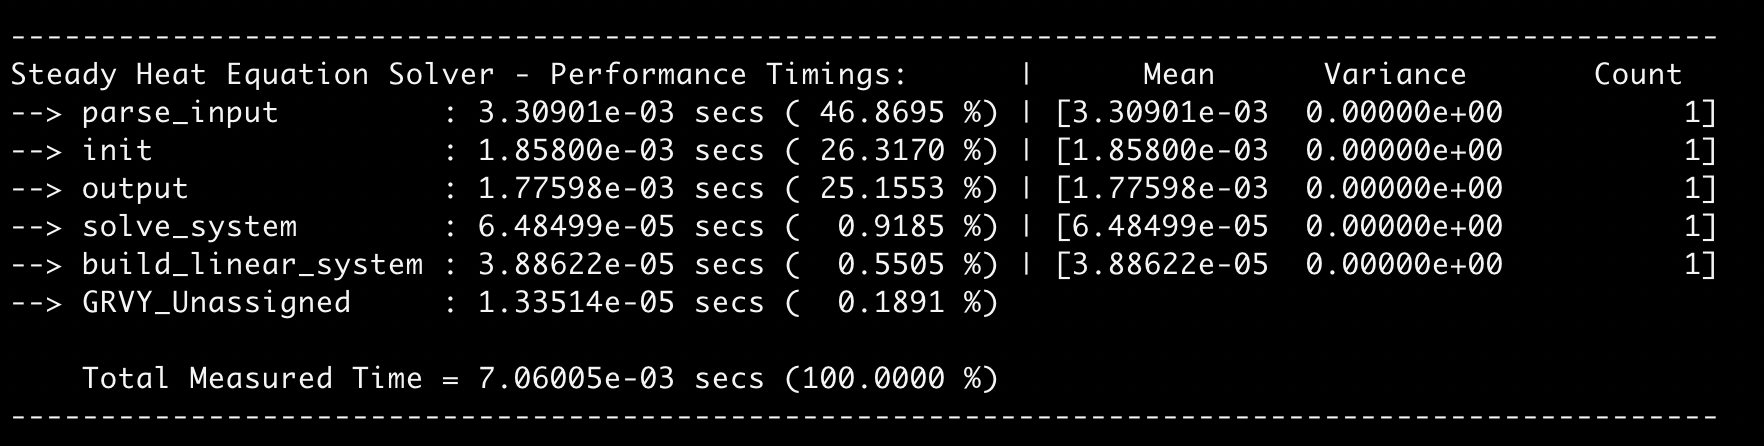
\includegraphics[width=0.9\textwidth]{runtime8.png}
\caption{\label{run8}Runtime summary for 8 points}
\end{figure}

\begin{figure}[htbp]
\centering
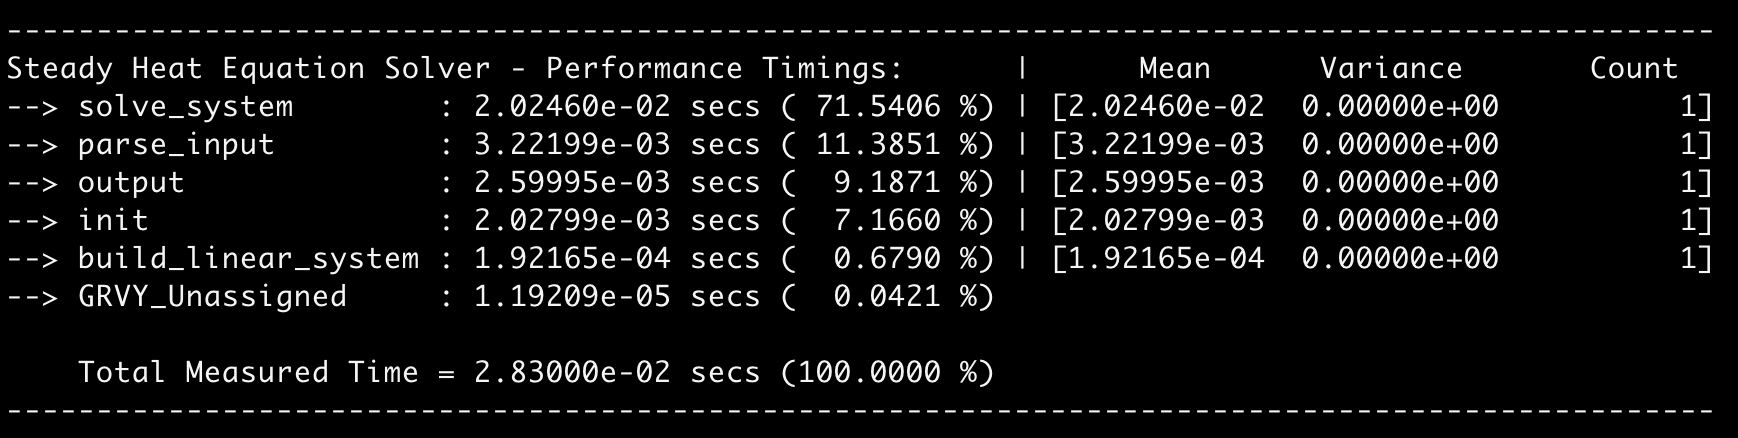
\includegraphics[width=0.9\textwidth]{run32.png}
\caption{\label{run32}Runtime summary for 32 points}
\end{figure}

\begin{figure}[htbp]
\centering
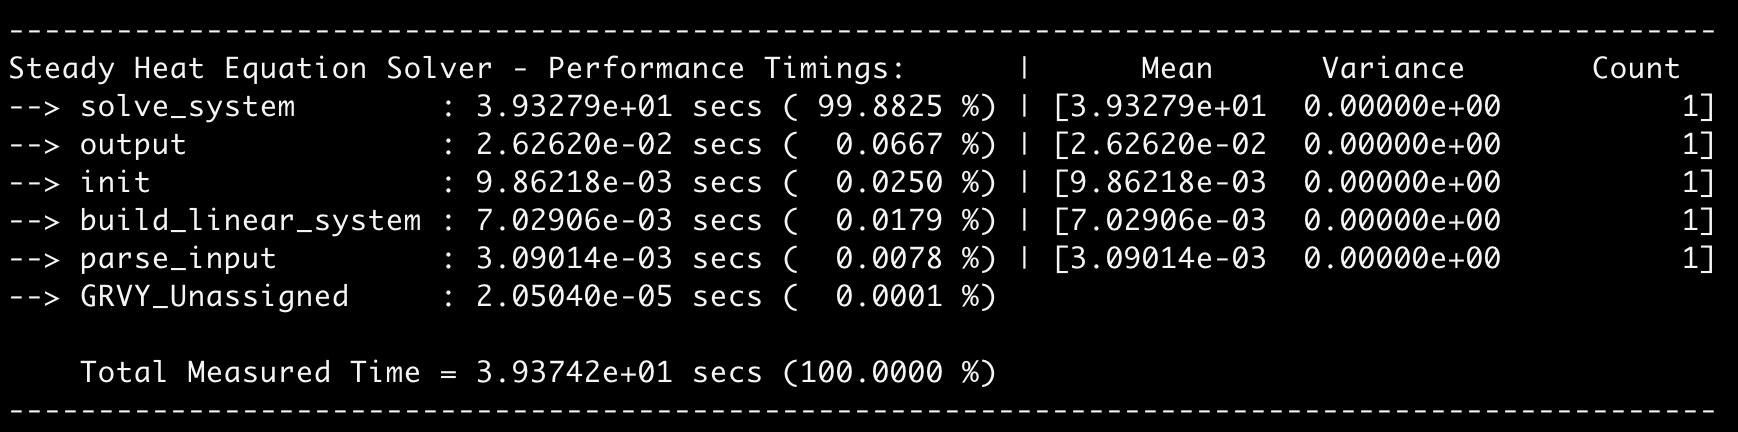
\includegraphics[width=0.9\textwidth]{run256.png}
\caption{\label{run256}Runtime summary for 256 points}
\end{figure}

\begin{table}[htbp]
\centering
\begin{tabular}{l|lll}
\hline
N / process\ \% & solve\_system & parse\_input & output \\
\hline
8  & 0.91 & 46.87  & 25.16\\
32  & 71.54  & 11.29 & 9.19\\
256 & 99.88 & 0.0078 & 0.0667\\
\hline
\end{tabular}
\caption{\label{table2}Runtime Summary}
\end{table}

\section{PETSC and Runtime Performance Comparison}
To use PETSC, you can just change the "iter\_method" to 3. I recommend you to use "mpirun" command as mentioned before to make sure it runs well. In Figure \ref{pet}, we can see that the time for 2D and $N = 128$ is still around $0.5s$, and the main usage is on PETSC\_Initialization.\\\\
For comparison, in 1D and 2D case, in Figure \ref{1dtime} and Figure \ref{2dtime} respectively, except for some starting points, as N grows, time for Jacobi and Gauss-Seidel grows as well. But for PETSC, the time for GMRES method is always around $0.4s-0.6s$, and it is not "very stable" depending on the initialization process. In 2D case, it is obivious that Jacobi and Gauss-Seidel arrive around $100s$. But using GMRES to solve cases for big N will save a lot of time with MPI and some preconditioners.\\\\
To reproduce the plots, you can run "\textbf{batch\_time.sh}" to get a directory called "\textbf{time\_record}" including all time performance results and use "\textbf{time\_record.m}" in MATLAB to get the plots.

\begin{figure}[htbp]
\centering
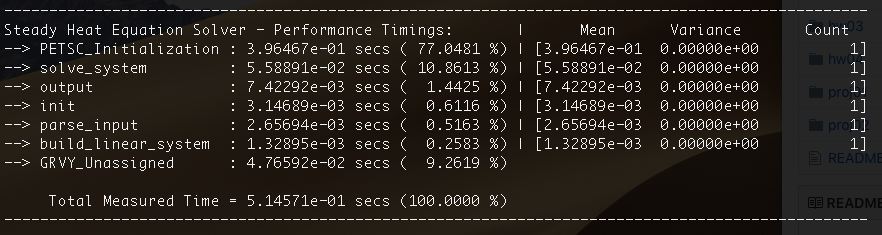
\includegraphics[width=0.85\textwidth]{pett.png}
\caption{\label{pet}Runtime Performance for PETSC, 2D, 4th order, N = 128}
\end{figure}

\begin{figure}[htbp]
\centering
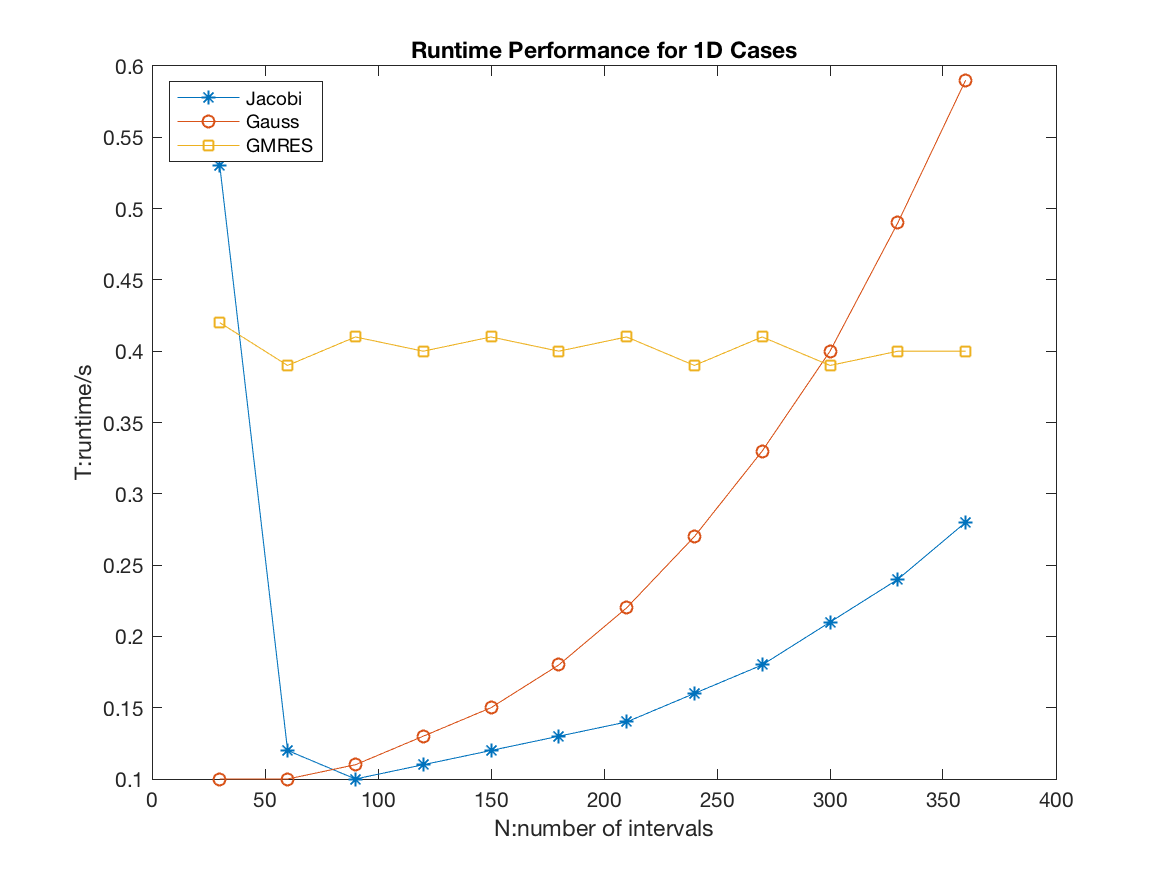
\includegraphics[width=0.85\textwidth]{1D_time.png}
\caption{\label{1dtime}Runtime Performance for 1D Cases}
\end{figure}

\begin{figure}[htbp]
\centering
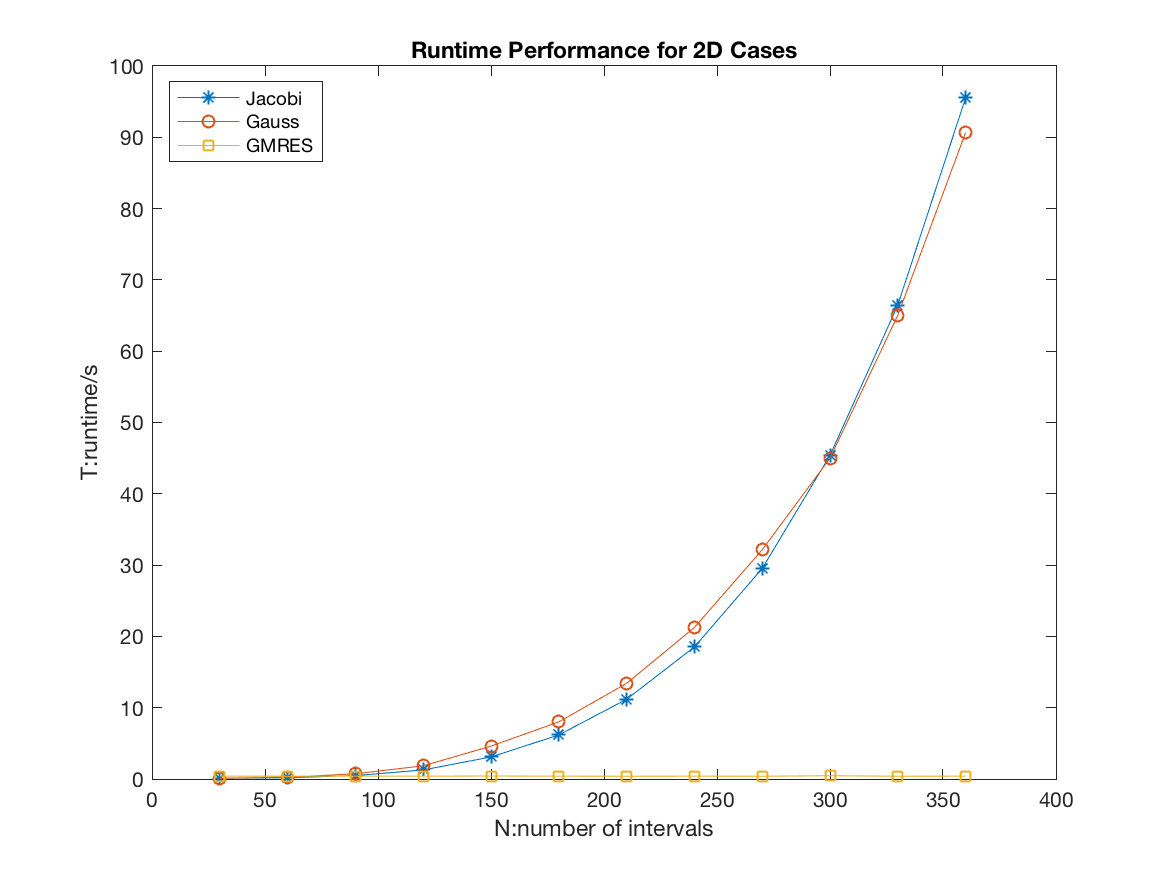
\includegraphics[width=0.85\textwidth]{2D_time.png}
\caption{\label{2dtime}Runtime Performance for 2D Cases}
\end{figure}


\section{Outputs and Tests with HDF5}
In the program, the output files are stored in HDF5 files. You can use "\textbf{h5dump [Filename]}" to see the datasets. You can use MATLAB, Python, and many tools to read h5 files and to plot with the data. I use MATLAB to plot the results. In test cases, I include all the test cases with reference h4 files and use "\textbf{h5diff}" to check the numerical differences.

\section{Solution Plots from HDF5}

We can visualize the solutions from hdf5 files using MATLAB. We can use "\textbf{heat\_plot2d.m}" to read data including coordinates: x and y, T\_sol and T\_exact in hdf5 file from "/test" directory or you can change the path to read the solution you get to visualize it into 3D plot (Figure \ref{2dsurf}) with "surf" and 2D plot (Figure \ref{2dcontour}) with "contourf". MATLAB code can also be get from Figure \ref{time_matlab}:

\begin{figure}[htbp]
\centering
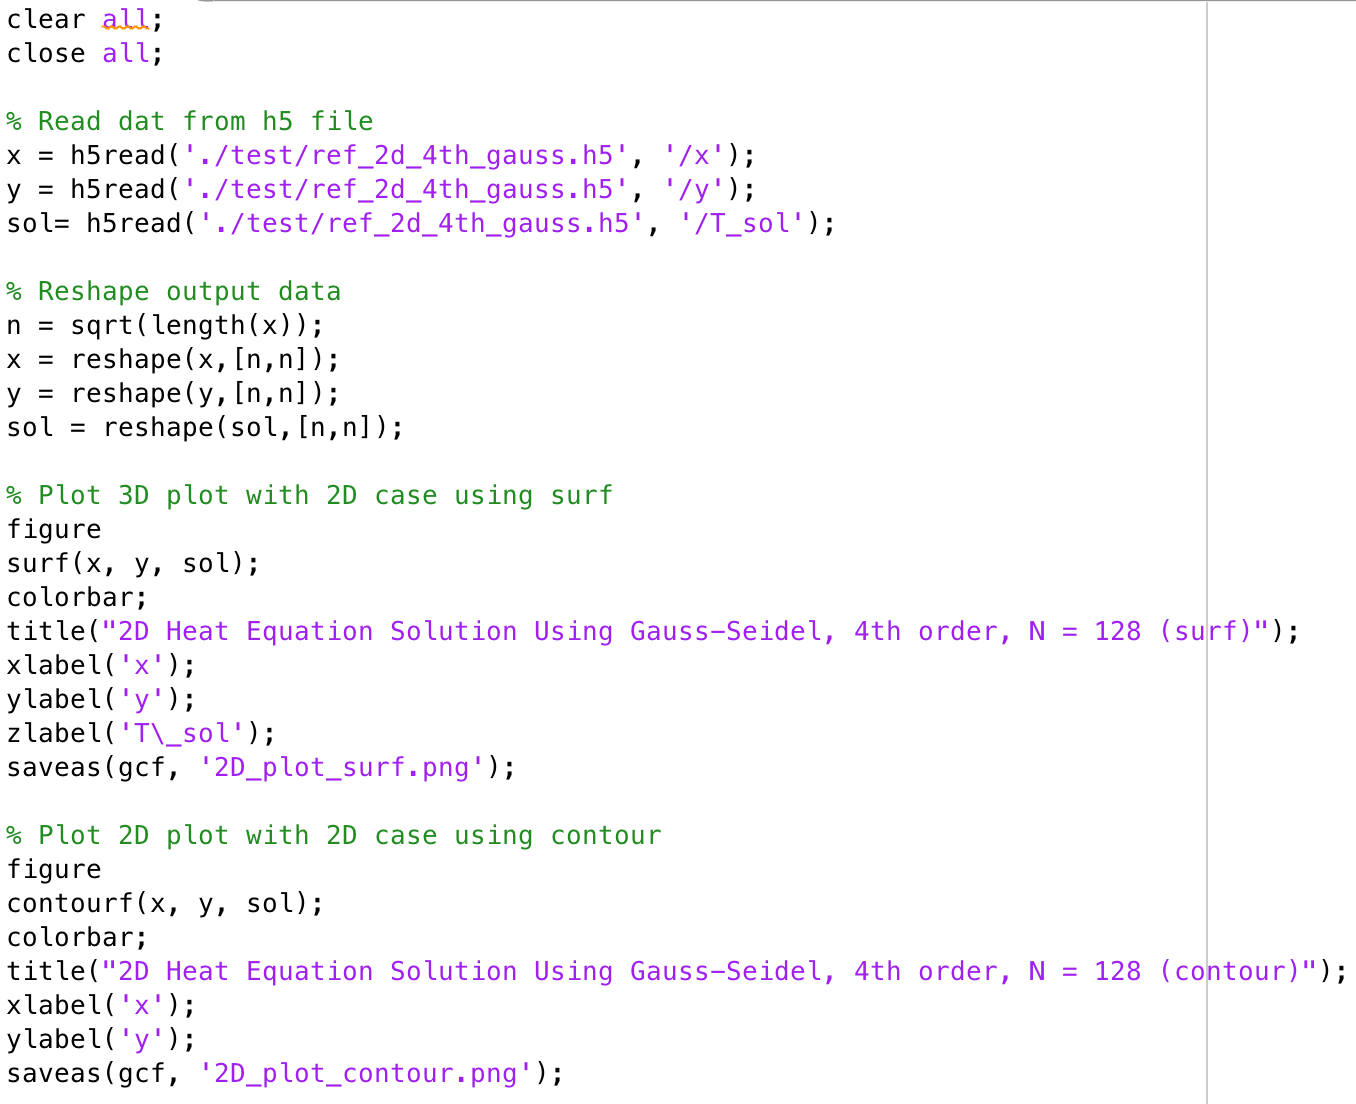
\includegraphics[width=0.85\textwidth]{mat.png}
\caption{\label{time_matlab}MATLAB Code for Plotting 2D case}
\end{figure}

\begin{figure}[htbp]
\centering
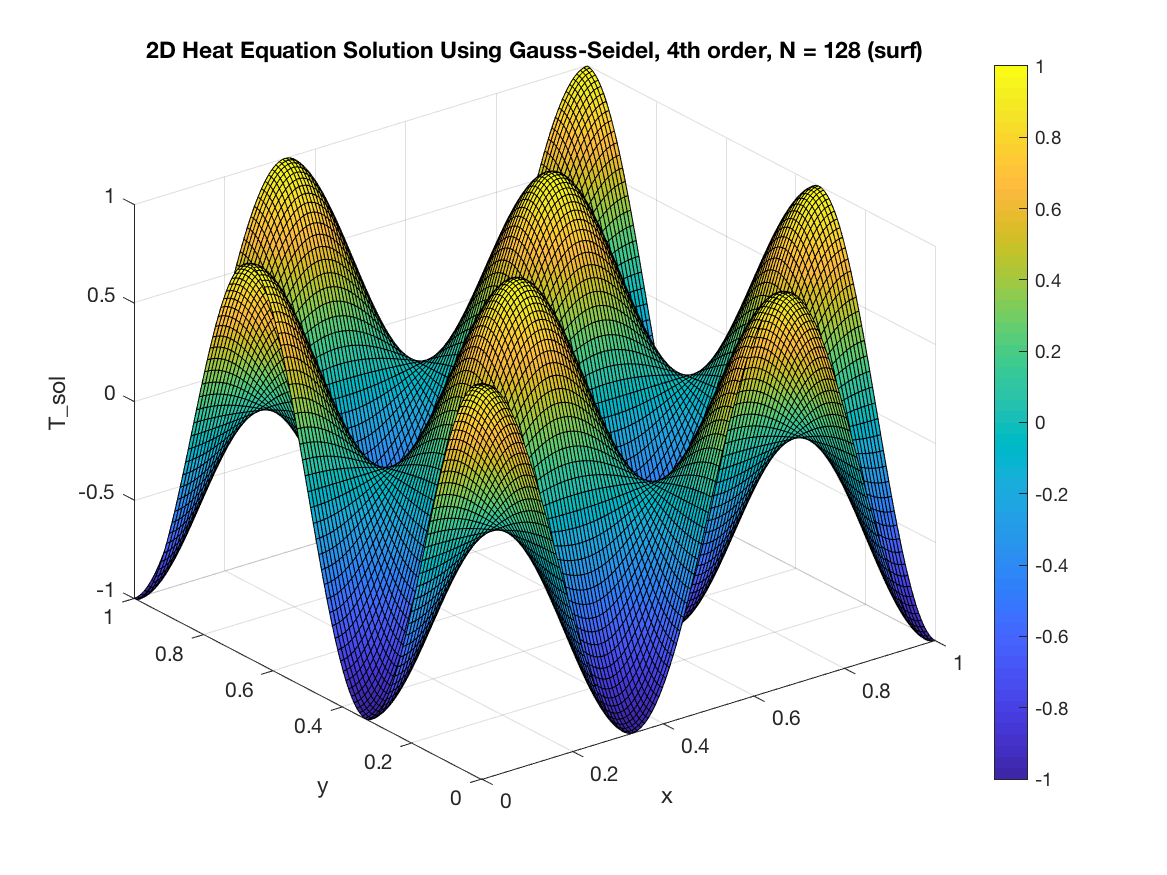
\includegraphics[width=0.85\textwidth]{2D_plot_surf.png}
\caption{\label{2dsurf}2D Solution Plot in 3D}
\end{figure}

\begin{figure}[htbp]
\centering
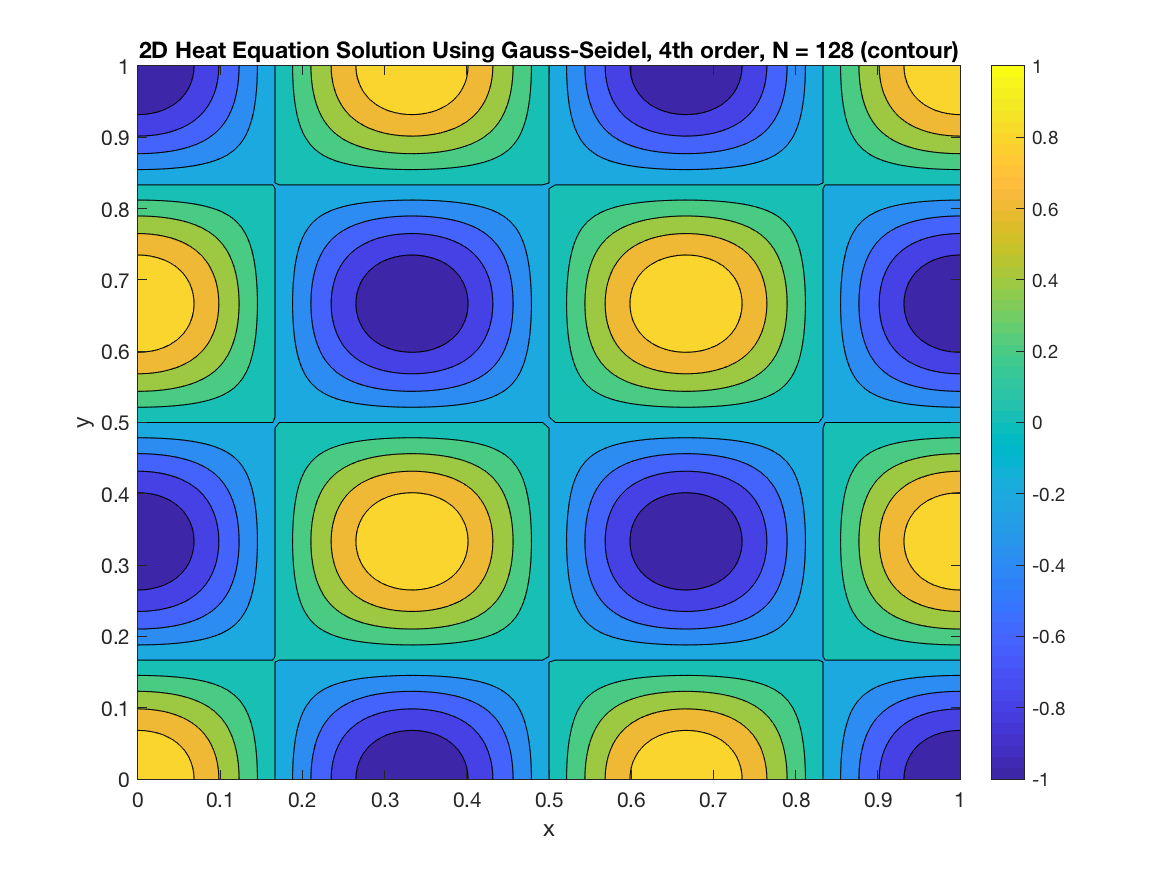
\includegraphics[width=0.85\textwidth]{2D_plot_contour.png}
\caption{\label{2dcontour}2D Solution Plot in 2D}
\end{figure}

\end{document}